\section{连续映射}
\label{sec:weak-continuous-mapping}

已知$X_n\xrightarrow{\mathrm{d}}X$，常常还要知道$X_n^{2}$、$\mathrm{e}^{X_n}$、$\mathbf{1}_{\{X_n>a\}}$或$1/X_n$的极限。对每个$X_n$作同一个确定的变换$g$，极限能否随之传递？若$g$连续，答案几乎写在定义里：对$f\in C_b$，复合$f\circ g$仍是有界连续函数，所以
\[
 \mathbb{E}\bigl[f(g(\bm{X}_n))\bigr]=\mathbb{E}\bigl[(f\circ g)(\bm{X}_n)\bigr]\longrightarrow\mathbb{E}\bigl[(f\circ g)(\bm{X})\bigr]=\mathbb{E}\bigl[f(g(\bm{X}))\bigr] .
\]

实际要用的$g$常有不连续点：阈值的示性函数在阈值处跳跃，倒数在$0$处没有定义。下面的定理允许$g$有不连续点，只要极限分布不把质量放在那里。

\begin{theorem}[连续映射定理]
\label{thm:weak-continuous-mapping}
设$\bm{X}_n\xrightarrow{\mathrm{d}}\bm{X}$，$\bm{X}_n,\bm{X}$取值于$\mathbb{R}^{d}$。设$g:\mathbb{R}^{d}\to\mathbb{R}^{k}$为Borel可测映射，$D_g$为它的不连续点集。若$\mathbb{P}(\bm{X}\in D_g)=0$，则$g(\bm{X}_n)\xrightarrow{\mathrm{d}}g(\bm{X})$。
\end{theorem}

\begin{proof}
可以证明$D_g$是Borel集，所以$\mathbb{P}(\bm{X}\in D_g)$有意义。用Portmanteau定理的(3)验证。取$\mathbb{R}^{k}$中的闭集$F$，记$\overline{g^{-1}(F)}$为原像的闭包。

先说明$\overline{g^{-1}(F)}\subset g^{-1}(F)\cup D_g$。设$\bm{x}$在闭包中，取$\bm{x}_m\in g^{-1}(F)$，$\bm{x}_m\to\bm{x}$。若$g$在$\bm{x}$处连续，则$g(\bm{x})=\lim g(\bm{x}_m)$，而$g(\bm{x}_m)\in F$，$F$闭，所以$g(\bm{x})\in F$，即$\bm{x}\in g^{-1}(F)$。否则$\bm{x}\in D_g$。

于是，由原像的闭包是闭集，以及$\bm{X}_n\xrightarrow{\mathrm{d}}\bm{X}$与Portmanteau定理的(3)，
\[
 \begin{aligned}
 \limsup_{n\to\infty}\mathbb{P}\bigl(g(\bm{X}_n)\in F\bigr)
 &\leq\limsup_{n\to\infty}\mathbb{P}\bigl(\bm{X}_n\in\overline{g^{-1}(F)}\bigr)
 \leq\mathbb{P}\bigl(\bm{X}\in\overline{g^{-1}(F)}\bigr)\\
 &\leq\mathbb{P}\bigl(\bm{X}\in g^{-1}(F)\bigr)+\mathbb{P}(\bm{X}\in D_g)=\mathbb{P}\bigl(g(\bm{X})\in F\bigr) .
 \end{aligned}
\]
再用一次Portmanteau定理即得结论。
\end{proof}

定理~\ref{thm:weak-continuous-mapping}通称\term{连续映射定理}（continuous mapping theorem）。条件$\mathbb{P}(\bm{X}\in D_g)=0$只涉及极限$\bm{X}$，与$\bm{X}_n$是否把质量放在$D_g$上无关。这与Portmanteau定理(5)的边界条件是同一种要求：示性函数$\mathbf{1}_A$的不连续点集正是$\partial A$。

\paragraph{阈值}
设$g(x)=\mathbf{1}_{\{x>1/2\}}$，$D_g=\{1/2\}$。对格点均匀分布，$U_n\xrightarrow{\mathrm{d}}U\sim\operatorname{Unif}(0,1)$，且$\mathbb{P}(U=1/2)=0$，所以$\mathbf{1}_{\{U_n>1/2\}}\xrightarrow{\mathrm{d}}\operatorname{Bern}(1/2)$。直接计算也是如此：$\mathbb{P}(U_n>1/2)=1-\lfloor n/2\rfloor/n\to1/2$。

换成$\delta_{1/n}\to\delta_0$与阈值$0$，$g(x)=\mathbf{1}_{\{x>0\}}$，则$g(1/n)=1$恒成立，而$g(0)=0$。极限分布的全部质量都在$D_g=\{0\}$上，条件不满足，结论确实失败。图~\ref{fig:weak-threshold-mapping}并列了这两种情形。

\begin{BookInlineFigure}
 \centering
 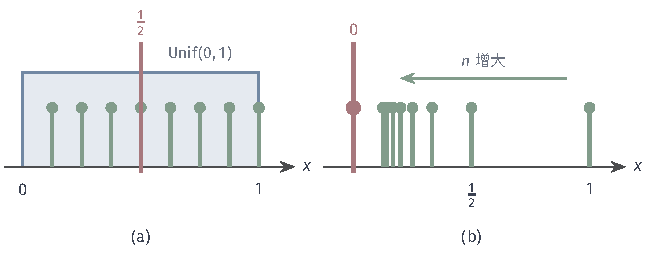
\includegraphics[width=110.6mm]{figures/07-probability/03-probability-limits/tikz/weak-threshold-mapping/figure.pdf}
 \caption{阈值映射与极限质量的位置。(a)格点均匀分布$U_8$的质点（绿）与极限$\operatorname{Unif}(0,1)$的密度（浅蓝），阈值$1/2$（红色竖线）处$U_8$有质量而极限没有，阈值右侧的概率收敛到$1/2$。(b)$\delta_{1/n}$的质点（绿）从右侧逼近阈值$0$，极限$\delta_0$（红点）恰好落在阈值上，$\mathbf{1}_{\{X_n>0\}}$恒为$1$，极限却是$0$。}
 \label{fig:weak-threshold-mapping}
\end{BookInlineFigure}

\paragraph{倒数}
令$g(x)=1/x$（$x\neq0$），$g(0)=0$，则$D_g=\{0\}$。若$X_n\xrightarrow{\mathrm{d}}X$且$\mathbb{P}(X=0)=0$，则$1/X_n\xrightarrow{\mathrm{d}}1/X$。$g(0)$取什么值无关紧要，它只影响$X_n=0$的样本，而极限分布不关心那里。

仍以格点均匀分布为例，$\mathbb{P}(U=0)=0$，所以$1/U_n\xrightarrow{\mathrm{d}}1/U$。极限的右尾为
\[
 \mathbb{P}(1/U>y)=\mathbb{P}(U<1/y)=\frac1y,\qquad y\geq1 ,
\]
这是第~\ref{chap:tail-probabilities}章参数为$1$的Pareto分布，没有期望。直接计算，$U_n<1/y$的格点是$k<n/y$，个数为$\lceil n/y\rceil-1$，于是
\[
 \mathbb{P}(1/U_n>y)=\frac{\lceil n/y\rceil-1}{n}\longrightarrow\frac1y .
\]
注意每个$1/U_n$都不超过$n$，有界；极限却是重尾分布。图~\ref{fig:weak-reciprocal}(a)画出这一收敛。

分母趋于零时条件就会失效。设$X_n=(-1)^{n}/n$，则$X_n\xrightarrow{\mathrm{d}}0$，极限把全部质量放在$D_g$上。$1/X_n=(-1)^{n}n$在$\pm\infty$之间来回跳，没有任何弱极限。即使取$X_n\sim\mathcal{N}(0,1/n^{2})$这样处处没有原子的分布，$1/X_n$的分布也是$1/X_1$的分布按$n$倍放大，质量逃向无穷远，见图~\ref{fig:weak-reciprocal}(b)。

\begin{BookInlineFigure}
 \centering
 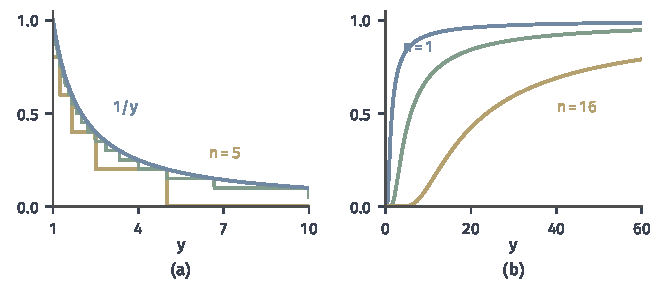
\includegraphics[width=112mm]{figures/07-probability/03-probability-limits/matplotlib/weak-reciprocal/figure.pdf}
 \caption{倒数映射。(a)$\mathbb{P}(1/U_n>y)$，$n=5$（黄）与$n=20$（绿），蓝线为极限$1/y$。(b)$X_n\sim\mathcal{N}(0,1/n^2)$时$\lvert1/X_n\rvert$的分布函数，$n=1$（蓝）、$4$（绿）、$16$（黄），曲线整体右移，质量逃向无穷远。}
 \label{fig:weak-reciprocal}
\end{BookInlineFigure}

连续映射定理处理的是同一个确定变换。若变换本身也随$n$变化，例如$g_n(x)=x+1/n$，则要另外论证；若变换涉及两个随机变量，例如$X_n+Y_n$，则需要$(X_n,Y_n)$作为一个随机向量的极限，这是下一节的问题。
